%!TEX root = ../report.tex
\documentclass[report.tex]{subfiles}
\begin{document}
    \chapter{Methodology}
        % Dont know where to put DATASET related content
    % One entire section could be my comparative study on multimodal dataset
    \section{Available Datasets}

    % \begin{itemize}
    %     \item The majority of deep multimodal perception approaches rely on supervised learning, and therefore necessitate multimodal datasets with labeled ground truth for training deep neural networks. While several multimodal datasets are available, many of these datasets are collected under clear weather conditions or do not include all sensors, such as cameras, LiDAR, and radar. Unfortunately, the availability of multimodal datasets collected under adverse weather conditions with all three sensors are limited. Table 1 summarizes some of the available multimodal datasets for evaluating the performance of deep multimodal perception techniques in adverse weather conditions. Of these datasets, only the recently released K-Radar \cite{Paek2022Jun} incorporates a high-resolution 4D-radar sensor. In the table, C-R-L-N-F denotes the Camera, Radar, LiDAR, Near-infrared, and Far-infrared sensors, respectively.
    %         \begin{table}[h]
    %             \centering
    %             \caption{List multimodal datasets with adverse weather conditions}
    %             \label{tab:my-table}
    %             \begin{tabular}{|l|l|l|l|}
    %                 \hline
    %                 \textbf{Name}       & \textbf{Sensors} & \textbf{Reference}               & \textbf{Year} \\ \hline
    %                 DENSE               & CRLNF            & \cite{bijelic2020seeing}    & 2020          \\ \hline
    %                 EU Long-term        & CRL              & \cite{yan2020eu}            & 2020          \\ \hline
    %                 nuScenes            & CRL              & \cite{caesar2020nuscenes}   & 2020          \\ \hline
    %                 The Oxford RobotCar & CRL              & \cite{barnes2020oxford}     & 2020          \\ \hline
    %                 RADIATE             & CRL              & \cite{sheeny2021radiate}    & 2021          \\ \hline
    %                 K-Radar             & CRL              & \cite{Paek2022Jun}          & 2022          \\ \hline
    %                 aiMotive            & CRL              & \cite{matuszka2022aimotive} & 2022          \\ \hline
    %                 Boreas              & CRL              & \cite{burnett2022boreas}    & 2022          \\ \hline
    %                 WADS                & CRLNF            & \cite{kurup2022winter}      & 2023          \\ \hline
    %             \end{tabular}
    %         \end{table}

    %         \begin{figure}[h]
    %             \centering
    %             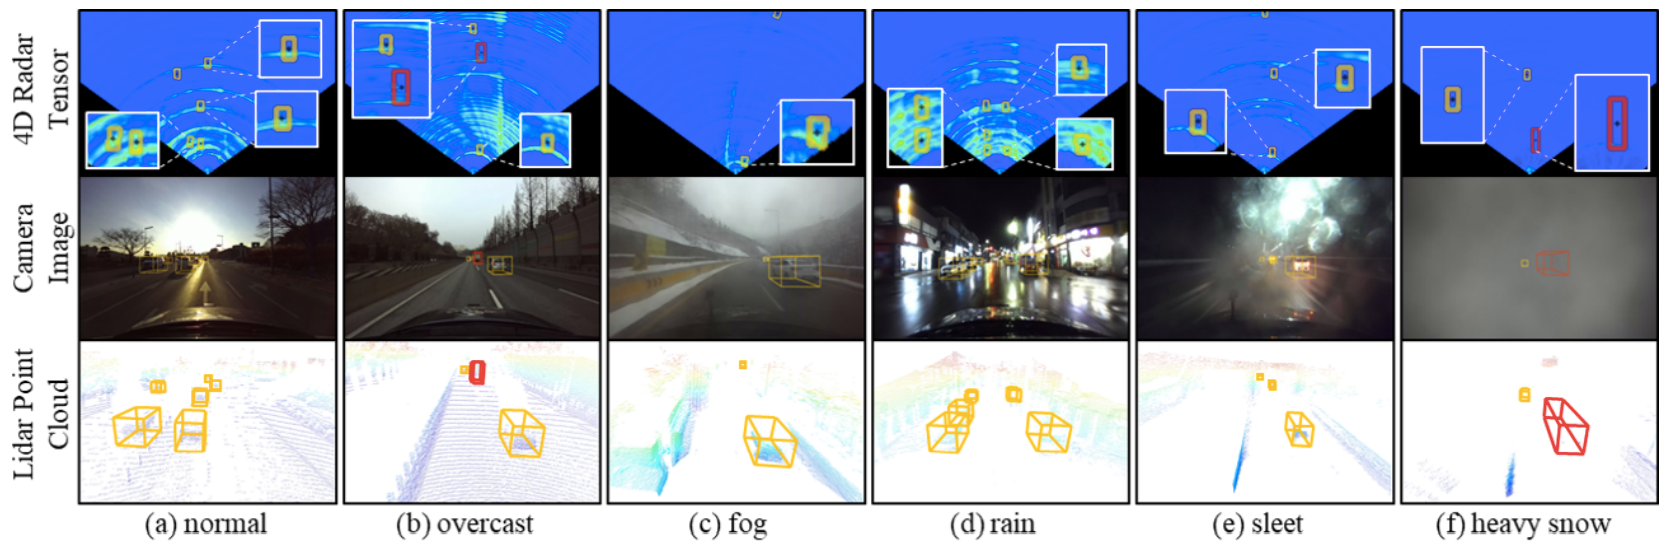
\includegraphics[width=1.0\textwidth]{images/all_sensors_in_adverse_weather.png}
    %             \caption{\centering Samples of K-Radar datasets for various weather conditions \cite{Paek2022Jun}}
    %             \label{fig:all_sensors_in_adverse_weather}
    %         \end{figure}
    %     \end{itemize}


    The majority of deep multimodal perception approaches rely on supervised learning, which necessitates the use of high-quality, large-scale multimodal datasets with labeled ground truth for training deep neural networks. Several multimodal datasets, such as KITTI \cite{geiger2012we}, ApolloScape \cite{huang2019apolloscape}, and Waymo \cite{sun2020scalability}, are prevalent in the domain of LiDAR-camera fusion. However, a significant number of these datasets are collected under clear weather conditions or lack a comprehensive array of sensors, including cameras, LiDAR, and Radar. A notable limitation is the scarcity of multimodal datasets that are collected under adverse weather conditions and incorporate at least all three of these essential sensors. Table \ref{datasets} summarizes some of the available multimodal datasets\footnote{For all the datasets, formal registration form is required to fill to access the dataset} for evaluating the performance of deep multimodal perception techniques in adverse weather conditions. The dataset are sorted in ascending order with respect to year.

    \begin{table}[!ht]
        \centering
        \caption{Multimodal Adverse Weather Conditions Datasets. Sensors†: C-R-L-N-F denote Camera, Radar, LiDAR, Near-infrared, and Far-infrared sensors, respectively. Weather Conditions‡: F-SN-R-O-SL-N denote Fog, Snow, Rain, Overcast, Sleet, and Night conditions, respectively. Note that highlighted datasets are used for the project.}
        \begin{tabular}{|l|l|l|l|l|l|l|}
        \hline
            \textbf{Name} & \textbf{Sensors†} & \textbf{Weather Cond.‡} & \textbf{Size (GB)} & \textbf{Year} & \textbf{Citation Cnt.} & \textbf{Reference} \\ \hline
            \textbf{DENSE} & \textbf{CRLNF} & \textbf{F, SN, R, O, N} & \textbf{582} & \textbf{2020} & \textbf{269} & \textbf{\cite{bijelic2020seeing}} \\ \hline
            \textbf{nuScenes} & \textbf{CRL} & \textbf{R, N} & \textbf{400} & \textbf{2020} & \textbf{3459} & \textbf{\cite{caesar2020nuscenes}} \\ \hline
            The Oxford RobotCar & CRL & R, SN, F & 4700 & 2020 & 317 & \cite{barnes2020oxford} \\ \hline
            EU Long-term & CRL & SN, R, O, N & NA & 2020 & 72 & \cite{yan2020eu} \\ \hline
            RADIATE & CRL & F, SN, R, O, SL, N & NA & 2021 & 132 & \cite{sheeny2021radiate} \\ \hline
            K-Radar & CRL & F, R, SN & 13000 & 2022 & 15 & \cite{Paek2022Jun} \\ \hline
            Boreas & CRL & SN, R, O, N & 4400 & 2022 & 38 & \cite{burnett2022boreas} \\ \hline
            aiMotive & CRL & R, O, N & 85 & 2023 & 3 & \cite{matuszka2022aimotive} \\ \hline
        \end{tabular}
        \label{datasets}
    \end{table}


    % The datasets for the project are selected based on the following criteria:
    % - Available Sensors, at least it should have camera, radar, and lidar
    % - Adverse weather conditions,
    % - Dataset documentation and accessibility,
    % - Usage by publicly available methods (so that comparison is possible)
    % - Perception Task, eg. Object Detection
    % - Radar datatype, the data should be available in point cloud format
    % - Time-synchronized and calibrated data

    % After considering above criteria, the following datasets are selected (also highlighted in the table): 
    % - DENSE
    % - nuScenes

    The selection of appropriate datasets is crucial. The criteria for selecting datasets cover several key areas, focusing on the availability of diverse sensors, specifically cameras, radar, and lidar, which are crucial for robust object detection in challenging environments. Additionally, the datasets must represent adverse weather conditions effectively, as this is a critical aspect of the research. Furthermore, the accessibility and thorough documentation of the datasets are considered, ensuring that the data can be easily understood and utilized in the research process. Another vital criterion is the dataset's popularity in existing research, as this allows for comparative analysis with publicly available methods, thereby validating the research findings. Moreover, the specific perception task, in this case, object detection, and the type of radar data, particularly in point cloud format, are essential considerations. The requirement for time-synchronized and calibrated data is also emphasized to ensure accuracy and reliability in sensor fusion and object detection algorithms.

    After a comprehensive evaluation of these criteria, two datasets have been chosen for this research: DENSE and nuScenes. The DENSE dataset is particularly suited for this study as it includes data from various sensors under adverse weather conditions, which is crucial for testing the efficacy of multimodal sensor fusion in challenging environments. The nuScenes dataset, on the other hand, is widely used in the field, providing a rich source of data with camera, radar, and lidar sensors. Its extensive use in the community allows for a meaningful comparison with existing methods. Both datasets provide time-synchronized and calibrated data, which is essential for the accuracy of object detection algorithms in adverse weather conditions. The selection of these datasets aligns perfectly with the research objectives, offering a comprehensive platform for exploring and advancing the capabilities of data-driven multimodal sensor fusion in object detection under challenging weather scenarios.

    \subsection{DENSE dataset \cite{bijelic2020seeing}}

    % The Dense dataset \cite{bijelic2020seeing} focused on evaluating multi-modal fusion algorithms under adverse weather. In addition to LiDAR and a stereo camera, it is also equipped with several all-weather sensors, including one frontal long-range radar, one gated camera working on the NIR band, one FIR camera, and one weather station sensor. The data are captured in various natural weather conditions, including rain, snow, light fog, and heavy fog, as well as in a controlled lab environment in a fog chamber. However, the dataset only provides sparse radar targets with limited FoV and low resolution. 
    % - The dataset is recorded in urban city, suburban, highway, and tunnel areas. 
    % - It coveres several weather conditions like light fog, dense fog, rain, snow, and night. The dataset is used by several multimodal sensor fusion publications for object detection. 
    % - Table \ref{tab:dataset_comparison} higlihts the sensor setup and dataset statistics for each dataset. 
    % - Geographical coverage of the data collection campaign covering two months and 10,000 km in Germany, Sweden, Denmark, and Finland. 
    % - DENSE dataset provides Radar targets in point cloud format.
    % - As Radar data points are inherently noisy, so the both datasets have already been preprocessed to remove the false points.
    % - Radar data directly provide 3D information consisting of range, azimuth, and velocity. As an additional note, new generation Radar sensors provide 4D data with range, azimuth, velocity, and elevation.
    % - It provides 2D annotations in COCO style format, where bbox format is x, y, width, height.
    The DENSE dataset, as detailed in Bijelic et al. (2020) \cite{bijelic2020seeing}, is a critical asset for evaluating multi-modal fusion algorithms in adverse weather conditions. Its standout feature is the extensive sensor array, including LiDAR, a stereo camera, a frontal long-range radar, a gated camera operating in the NIR band, a FIR camera, and a weather station sensor, as illustrated in Figure \ref{fig:dense_test_vehicle_setup}. These sensors allow for detailed data capture under various adverse weather conditions, such as rain, snow, light fog, and dense fog. Notably, the DENSE dataset uniquely offers a split for light and dense fog conditions, essential for assessing the detection performance of Lidar and Radar in varying visibility scenarios. The range of these conditions and their distribution are visually depicted in Figure \ref{fig:dense_distribution_of_weather_conditions}. Additionally, the dataset includes data from a controlled lab environment within a fog chamber, offering a distinct view of sensor performance under simulated conditions. However, it's important to note that for the purposes of this project, only real-world data from the DENSE dataset is utilized.

    The dataset covers a broad spectrum of environments, encompassing urban cities, suburban areas, highways, and tunnels. Its geographical scope is extensive, with data collection spanning over two months and covering 10,000 km across Germany, Sweden, Denmark, and Finland. This diverse environmental range enhances the dataset's applicability in various real-world scenarios.

    Technically, the DENSE dataset offers radar targets in a point cloud format, aligning well with the Lidar data. Given the inherent noise in radar data, preprocessing has been performed to eliminate false points, thereby bolstering the dataset's accuracy and reliability. The radar data includes 3D information - range, azimuth, and velocity. Moreover, it's noteworthy that the latest generation of radar sensors in the dataset provides 4D data, adding elevation to the existing dimensions. There are total 3 classes available in the dataset, including car, pedestrian, and cyclist. Object annotations in the DENSE dataset are provided in the COCO style format, with bounding box (bbox) parameters specified as x, y, width, and height. The annotation processed is well described in the supplementary material from the paper \cite{heide2023adverseweatherfusion}. This meticulous approach to data collection, processing, and annotation positions the DENSE dataset as a powerful and adaptable tool for research in adverse weather conditions, especially in the domain of data-driven multimodal sensor fusion.

        % \begin{figure}[h]
        %         \centering
        %         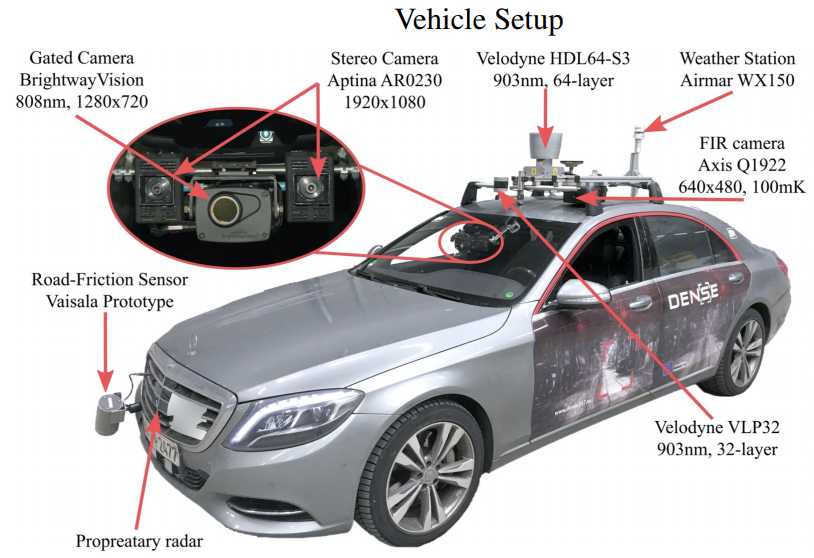
\includegraphics[width=0.5\textwidth]{images/datasets/dense/test_vehicle_setup.png}
        %         \caption{Test Vehicle Setup \cite{bijelic2020seeing}}
        %         \label{fig:dense_test_vehicle_setup}
        % \end{figure}

        % \begin{figure}[h]
        %         \centering
        %         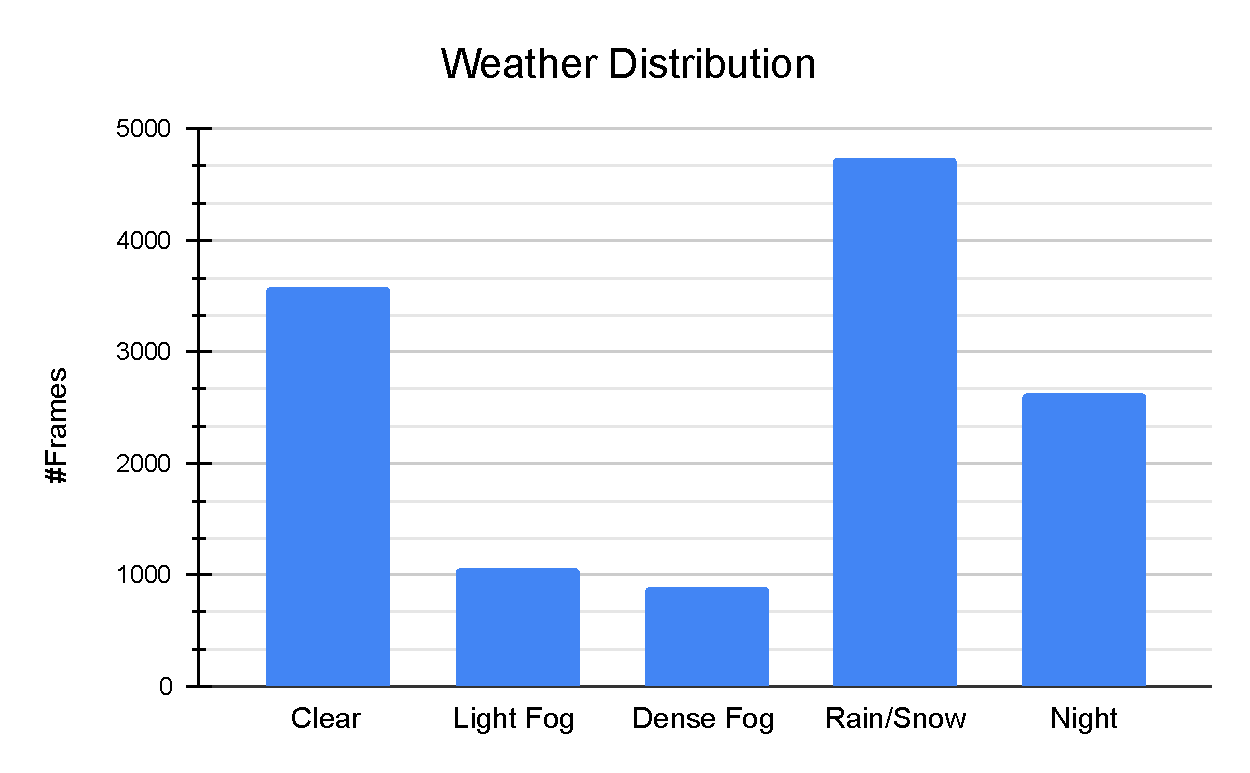
\includegraphics[width=0.5\textwidth]{images/datasets/dense/distribution_of_weather_conditions.pdf}
        %         \caption{Distribution of Weather Conditions \cite{bijelic2020seeing}}
        %         \label{fig:dense_distribution_of_weather_conditions}
        % \end{figure}

        \begin{figure}[h]
            \centering
            \begin{minipage}{0.45\textwidth}
                \centering
                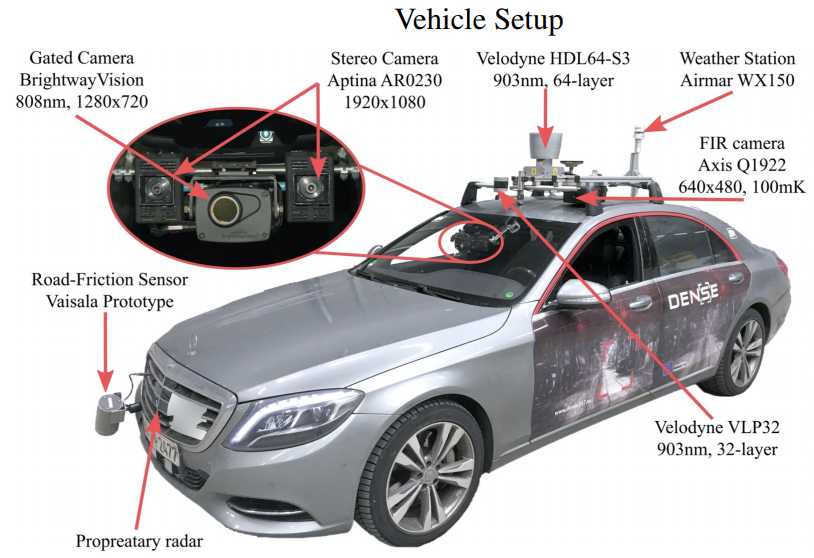
\includegraphics[width=\textwidth]{images/datasets/dense/test_vehicle_setup.png}
                \caption{Test Vehicle Setup \cite{bijelic2020seeing}}
                \label{fig:dense_test_vehicle_setup}
            \end{minipage}
            \hfill
            \begin{minipage}{0.45\textwidth}
                \centering
                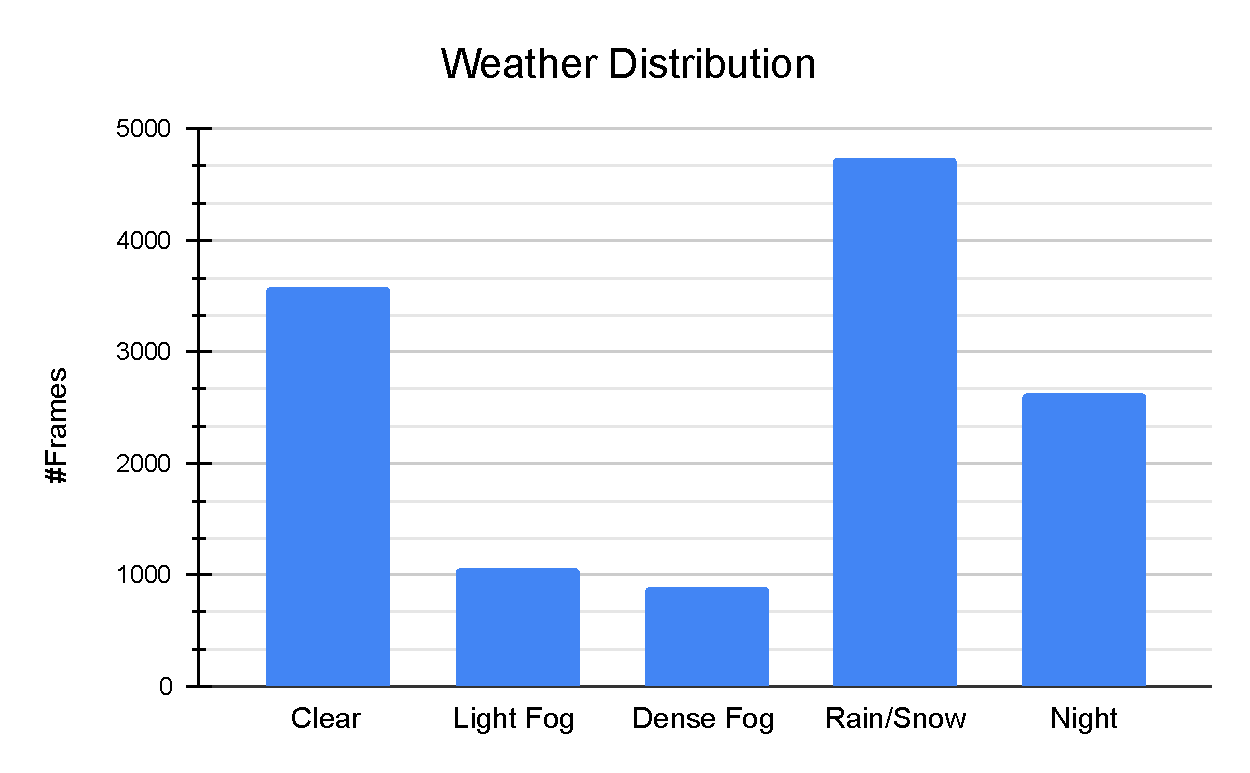
\includegraphics[width=\textwidth]{images/datasets/dense/distribution_of_weather_conditions.pdf}
                \caption{Distribution of Weather Conditions \cite{bijelic2020seeing}}
                \label{fig:dense_distribution_of_weather_conditions}
            \end{minipage}
        \end{figure}
        

        TODO: add Classwise distribution
        % \begin{figure}[h]
        %     \centering
        %     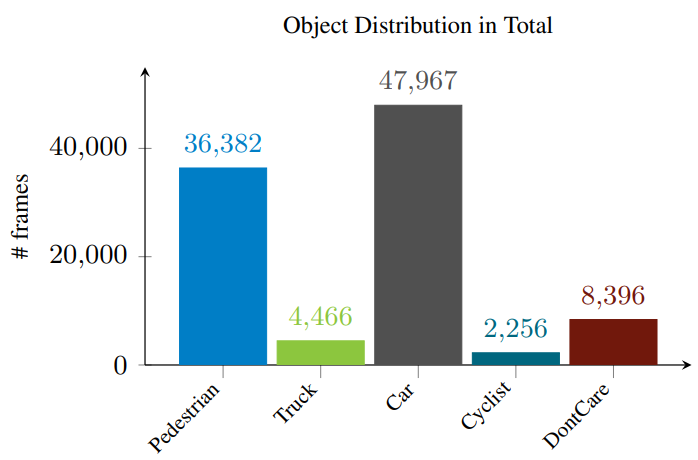
\includegraphics[width=0.9\textwidth]{images/datasets/dense/classwise_distribution.png}
        %     \caption{Classwise Distribution \cite{bijelic2020seeing}}
        %     \label{fig:dense_classwise_distribution}
        % \end{figure}

        TODO: put two in 4x4 grid, random samples of the dataset, one for clean and other with adverse weather conditions 


    \subsection{nuScenes dataset \cite{caesar2020nuscenes}}

    % NuScenes \cite{caesar2020nuscenes} is the most popular dataset for its large-scale and diverse scenarios. The capturing vehicle is equipped with a 32-beam LiDAR, 6 cameras, 5 long-range multi-mode radars, and a GPS/IMU system. It provides 3D annotations of 23 classes of road users in 1000 scenes, with a total of 1.3 million frames. 
    % - Although, the Radar used in nuScenes has a sparse data, but it is good dataset to start with and also well documented. 
    % - The dataset is recorded in urban city, suburban, and highway areas.
    % - It coveres less adverse weather conditions compared to DENSE dataset, like rain and night.
    % - Table \ref{tab:dataset_comparison} higlihts the sensor setup and dataset statistics in comparison to DENSE.
    % - Geographical coverage of the data collection campaign covering 242 km in Boston and Singapore.
    % - It provides Radar targets in point cloud format same as DENSE dataset.
    % - Note that nuscenes dataset doesn't provide 2D annotations so the individual methods create their own 2D annotations based on the 3D annotations.
    % - After creating 2D annotations, the dataset is converted to COCO style format, where bbox format is x, y, width, height.

    In addition to the DENSE dataset, this project also uses the nuScenes dataset \cite{caesar2020nuscenes} as a benchmark. The nuScenes dataset stands out for its large-scale and diverse scenarios. The data collection vehicle for nuScenes, as depicted in Figure \ref{fig:nuscenes_test_vehicle_setup}, is equipped with a comprehensive set of sensors, including a 32-beam LiDAR, six cameras, five long-range multi-mode radars, and a GPS/IMU system. This dataset provides 3D annotations for 23 classes of road users across 1,000 scenes, accumulating to a total of 1.3 million frames. Although the radar data in nuScenes is sparse, its extensive documentation makes it a good starting point for research in object detection.

    The nuScenes dataset focuses on urban, suburban, and highway areas, but it covers fewer adverse weather conditions compared to the DENSE dataset, primarily rain and night scenarios, as shown in Figure \ref{fig:nuscenes_distribution_of_weather_conditions}. Like DENSE, nuScenes also provides radar data in point cloud format. There are total 10 classes in the dataset, including car, truck, trailer, bus, construction vehicle, bicycle, motorcycle, pedestrian, traffic cone, and barrier. However, a notable distinction is that nuScenes does not provide 2D annotations. Researchers using this dataset typically generate their own 2D annotations based on the 3D annotations provided. Once these 2D annotations are created, the data is converted into the COCO style format, similar to DENSE, where the bbox format includes x, y, width, and height dimensions.


        % \begin{figure}[h]
        %     \centering
        %     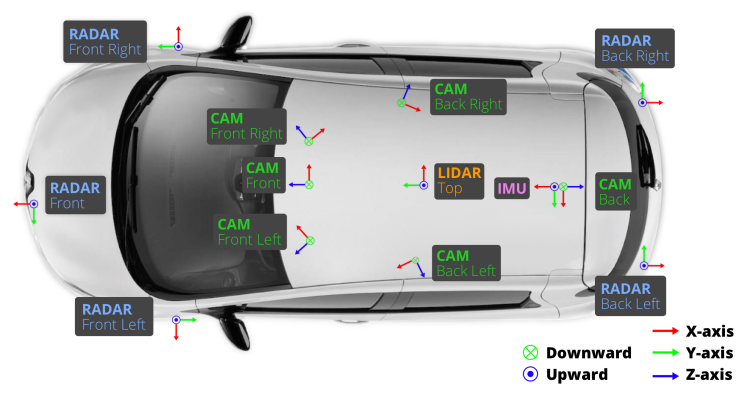
\includegraphics[width=0.9\textwidth]{images/datasets/nuscenes/test_vehicle_setup.png}
        %     \caption{Test Vehicle Setup \cite{bijelic2020seeing}}
        %     \label{fig:nuscenes_test_vehicle_setup}
        % \end{figure}

        % \begin{figure}[h]
        %     \centering
        %     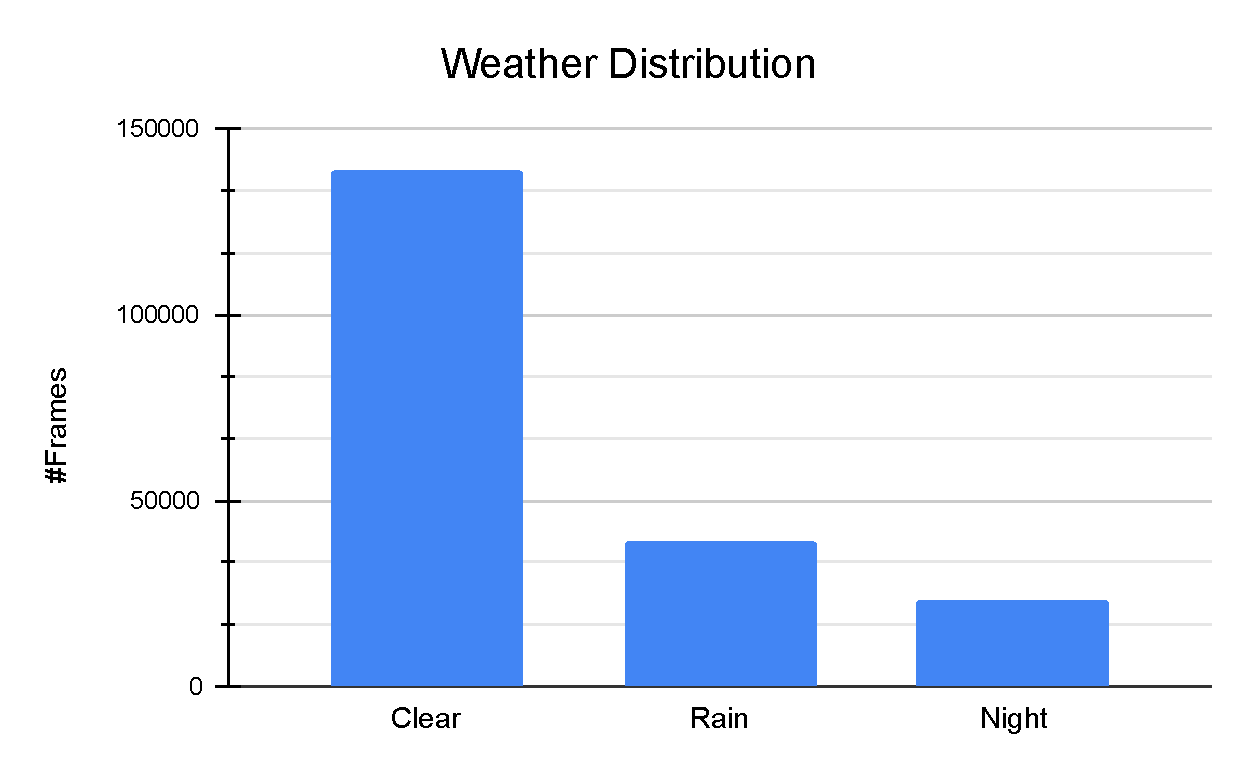
\includegraphics[width=0.9\textwidth]{images/datasets/nuscenes/distribution_of_weather_conditions.pdf}
        %     \caption{Distribution of Weather Conditions \cite{bijelic2020seeing}}
        %     \label{fig:nuscenes_distribution_of_weather_conditions}
        % \end{figure}

        \begin{figure}[h]
            \centering
            \begin{minipage}{0.48\textwidth}
                \centering
                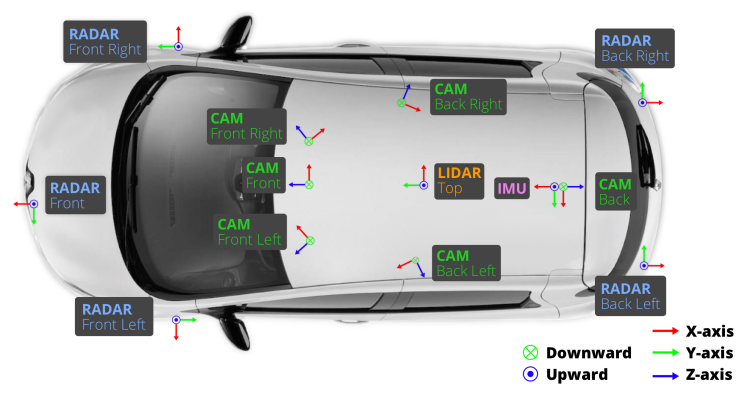
\includegraphics[width=\textwidth]{images/datasets/nuscenes/test_vehicle_setup.png}
                \caption{Test Vehicle Setup \cite{caesar2020nuscenes}}
                \label{fig:nuscenes_test_vehicle_setup}
            \end{minipage}
            \hfill
            \begin{minipage}{0.48\textwidth}
                \centering
                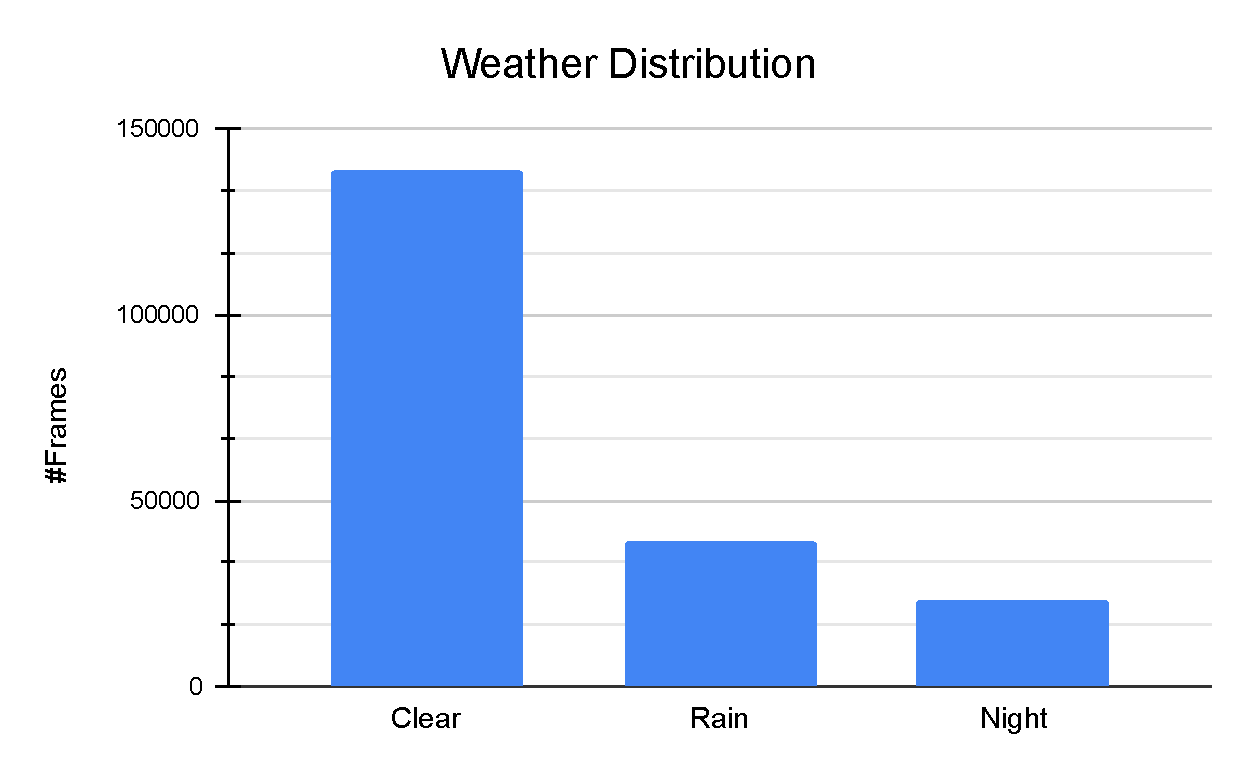
\includegraphics[width=\textwidth]{images/datasets/nuscenes/distribution_of_weather_conditions.pdf}
                \caption{Distribution of Weather Conditions \cite{caesar2020nuscenes}}
                \label{fig:nuscenes_distribution_of_weather_conditions}
            \end{minipage}
        \end{figure}
        

        TODO: add Classwise distribution
        % \begin{figure}[h]
        %     \centering
        %     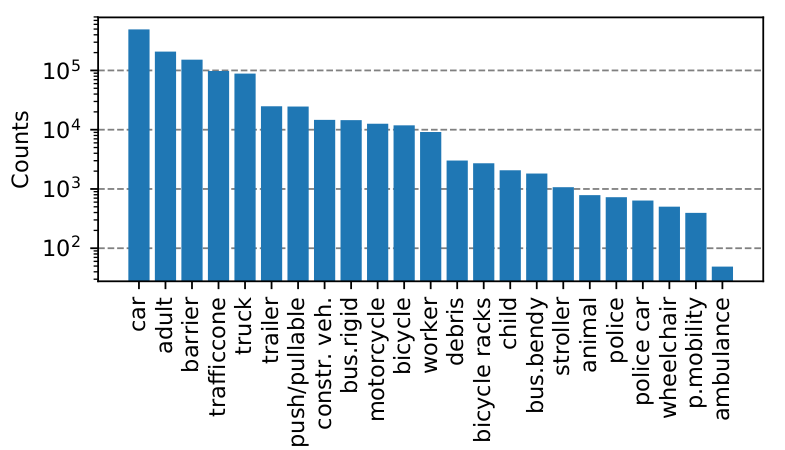
\includegraphics[width=0.9\textwidth]{images/datasets/nuscenes/classwise_distribution.png}
        %     \caption{Classwise Distribution \cite{bijelic2020seeing}}
        %     \label{fig:nuscenes_classwise_distribution}
        % \end{figure}
        TODO: put two in 4x4 grid, random samples of the dataset, one for clean and other with adverse weather conditions

        Table \ref{tab:dataset_comparison} highlights the overall comparison of the sensor setup and dataset statistics for datasets used in this project.

        \begin{table}[h!]
            \centering
            \caption{Comparison of Dataset Features}
            \begin{tabular}{|l|c|c|}
              \hline
              \textbf{Dataset} & \textbf{NuScenes \cite{caesar2020nuscenes}} & \textbf{DENSE \cite{bijelic2020seeing}} \\
              \hline
              Sensor Setup & 6 & 2 \\
              RGB Cameras & 6 & 2 \\
              RGB Resolution & 1600x900 & 1920x1024 \\
              Lidar Sensors & 1 & 2 \\
              Lidar Resolution & 32 & 64 \\
              Radar Sensor & 4 & 1 \\
              Gated Camera & x & 1 \\
              FIR Camera & x & 1 \\
              Frame Rate & 1 Hz/10 Hz & 10 Hz \\
              \hline
              \textbf{Dataset Statistics} &  &  \\
              \hline
              Labeled Frames & 40K & 13.5K \\
              Labels & 1.4M & 100K \\
              Scene Tags & \checkmark & \checkmark \\
              Night Time & \checkmark & \checkmark \\
              Light Weather & \checkmark & \checkmark \\
              Heavy Weather & x & \checkmark \\
              Fog Chamber & x & x \\
              \hline
            \end{tabular}
            \label{tab:dataset_comparison}
          \end{table}


    \section{Setup}

    \section{Experimental Design}

    \section{Evaluation Metrics}

    

\end{document}
